%%for slideshow
\documentclass[ignorenonframetext]{beamer} %add option 'draft' for quicker compilation
\usepackage{amsmath,amssymb,multirow}
\newcommand{\slides}{1}
%this only compiles frames with [label=current]
%\includeonlyframes{current} 
 
%for handouts
%\documentclass[a4paper,12pt]{article}
%\usepackage{beamerarticle}
%\newcommand{\slides}{0}

\mode<presentation>{
% for theme info see:
% http://www.ctan.org/tex-archive/macros/latex/contrib/beamer/doc/beameruserguide.pdf
\usetheme{default}
  \setbeamercovered{transparent}
  %Add university logo
  %\pgfdeclareimage[height=1cm]{university-logo}{logo}
  %\logo{\pgfuseimage{university-logo}}
  % If you wish to uncover everything in a step-wise fashion, uncomment
  % the following command:
%  \beamerdefaultoverlayspecification{<+->}

% get rid of navigation panel
\setbeamertemplate{navigation symbols}{} 

	\newcommand{\tcr}{\textcolor{red}}
}
\mode<article>{
  \usepackage{fullpage}
	\newcommand{\tcr}{\textcolor{black}}
  \renewcommand{\baselinestretch}{1.0}
  \oddsidemargin -1.5cm \evensidemargin -1.5in
  \topmargin=-1.5cm \headheight=0pt
  \headsep 0pt \textwidth=19cm
  \textheight=27cm \columnsep 10pt \columnseprule 0pt \parindent 0pt
  \parskip 0.0pt
  \usepackage{tweaklist}
  \renewcommand{\itemhook}{
    \setlength{\topsep}{-0pt}
    \setlength{\itemsep}{-0pt}
    \setlength{\parsep}{-0pt}
  }
  \renewcommand{\enumhook}{
    \setlength{\topsep}{-0pt}
    \setlength{\itemsep}{-0pt}
    \setlength{\parsep}{-0pt}
  }
}

\usepackage[english]{babel}
\usepackage[latin1]{inputenc}
\usepackage{helvet}
\renewcommand*\familydefault{\sfdefault} %% Only if the base font of the document is to be sans serif
%\usepackage{times}
\usepackage[T1]{fontenc}
\usepackage{graphics,graphicx,fancyhdr,color,amsmath,url,enumerate,alltt}
\usepackage{epsf}
\usepackage{ifthen}


\newcommand{\bc}{\begin{center}}
\newcommand{\ec}{\end{center}}
\newcommand{\bn}{\begin{enumerate}}
\newcommand{\en}{\end{enumerate}}
\newcommand{\bi}{\begin{itemize}}
\newcommand{\ei}{\end{itemize}}
\newcommand{\be}{\begin{eqnarray}}
\newcommand{\ee}{\end{eqnarray}}
\newcommand{\bes}{\begin{eqnarray*}}
\newcommand{\ees}{\end{eqnarray*}}
\newcommand{\expect}[1]{\mathbb{E}\left[ #1 \right]}


\title[Smoothing over complex regions]{Multidimensional scaling as a tool for smoothing over complex spatial regions}

\author[Miller]{David Lawrence Miller}

\institute{Mathematical Sciences\\University of Bath}

%\date[23-25 June 2009] {Modelling complex environmental spatial and temporal data, University of Bath}
%\date[July 2009] {useR! 2009, Rennes}
%\date[September 2009] {CREEM Seminar, 23 September 2009}
%\date[July 2010] {International Statistical Ecology Conference, 6-9 July 2010}
% PDRA interview, St Andrews 18 Jan 2011


% - Either use conference name or its abbreviation.
% - Not really informative to the audience, more for people (including
%   yourself) who are reading the slides online

% Delete this, if you do not want the table of contents to pop up at
% the beginning of each subsection:
\mode<presentation> {
%    \AtBeginSubsection[]
    \AtBeginSection[]
    {
    \begin{frame}<beamer>
        \frametitle{Outline}
        %\tableofcontents[currentsection,currentsubsection]
        \tableofcontents[currentsection]
    \end{frame}
    }
}
\begin{document}

\begin{frame}
  \titlepage
\end{frame}

\mode<article>{
\maketitle
}

\mode<presentation> {
\begin{frame}
  \frametitle{Outline}
  \tableofcontents %[pausesections]
  % You might wish to add the option [pausesections]
\end{frame}
}

\section{Smoothing over complex regions}

\subsection{The problem}

\begin{frame}
	\frametitle{Smoothing in 2 dimensions}
       \bi
         \item Have some geographical region and wish to find out something about the biological population in it. 
         \item Response is eg. animal distribution, wish to predict based on $(x,y)$ and other covariates eg. habitat, size, sex, etc.
         \item This problem is relatively easy if the domain is simple.
       \ei
       \bc
         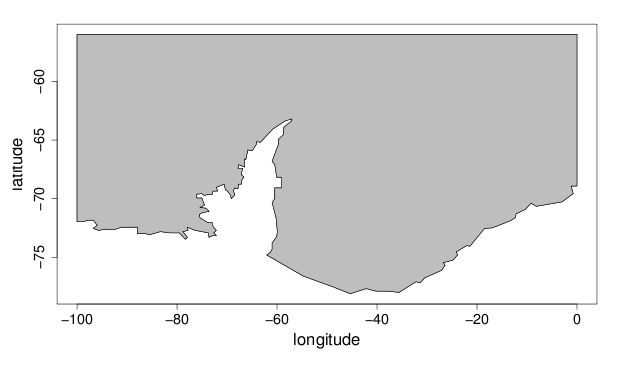
\includegraphics[width=2.5in]{figs/peninsula.png}
       \ec
\end{frame}

\begin{frame}
	\frametitle{Leakage (or, ``whales don't live in glaciers'')}
       \bi
         \item Smoothing of complex domains makes this a lot more difficult.
         \item Problem of leakage.
         \item Wrong metric.
         \item Euclidean distance doesn't always make sense.
       \ei
       \bc\begin{tabular}{@{}cc}
          & \\
          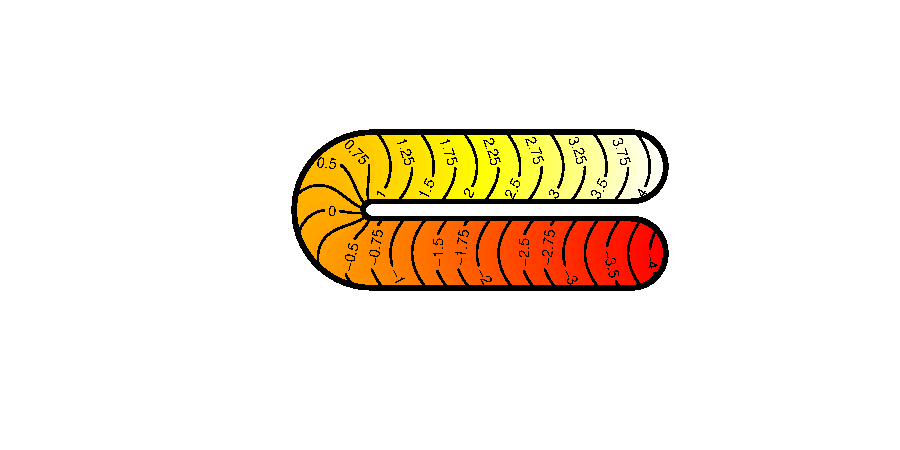
\includegraphics[width=2in, trim=1in 1in 1in 1in]{figs/ramsayhorseshoe} & 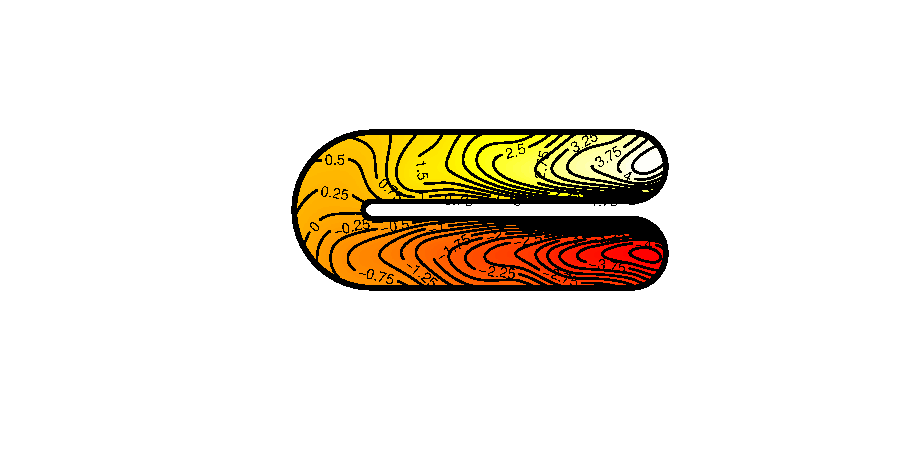
\includegraphics[width=2in, trim=1in 1in 1in 1in]{figs/leakageexample}\\
          (modified) Ramsay test function & Thin plate spline fit\\
       \end{tabular}\ec
\end{frame}

\subsection{Smoothing with splines}

\begin{frame}
	\frametitle{Smoothing with penalties}
      \bi
        \item Do smoothing with splines in an additive model framework.
        \item Take some linear combination of (known) basis functions.
        \item Penalize based on integral of second squared derivative:
            \begin{equation*}
	            \int\int_\Omega \Big( \Big(\frac{\partial^2 f(x,y)}{\partial x^2}\Big)^2 + \Big(\frac{\partial^2 f(x,y)}{\partial x \partial y}\Big)^2 + \Big(\frac{\partial^2 f(x,y)}{\partial y^2}\Big)^2\Big) \text{d}x\text{d}y.
            \end{equation*}
        \item Here using thin plate regression splines (eg Wood (2003)).
        \includegraphics[width=4in]{figs/tprsex} 
      \ei
\end{frame}


%\begin{frame}
%	\frametitle{Smoothing with penalties}
%      \bi
%         \item Objective function takes the form:
%      \ei
%      \bc
%      \begin{equation*}
%      \sum_{i=1}^n (z_i-\hat{f}(x_i,y_i;\hat{\theta}))^2 + \lambda \int_\Omega Pf(x,y;\hat{\theta})d\Omega
%      \end{equation*}
%      \ec
%      \bi
%         \item $\hat{f}$ is the function you want to estimate, made up of some combination of basis functions.
%         \item $P$ is some squared derivative penalty operator, usually $P=(\frac{\partial^2}{\partial x^2}+\frac{\partial^2}{\partial y^2})^2$.
%         \item This can be generalized to an additive model or GAM.
%      \ei
%\end{frame}
%
%\begin{frame}
%	\frametitle{Basis functions}
%       \bi
%       	  \item Fall into two classes: knot- and eigen-based.
%         \item P-splines (Marx and Eilers, 1996)
%          \bc
%         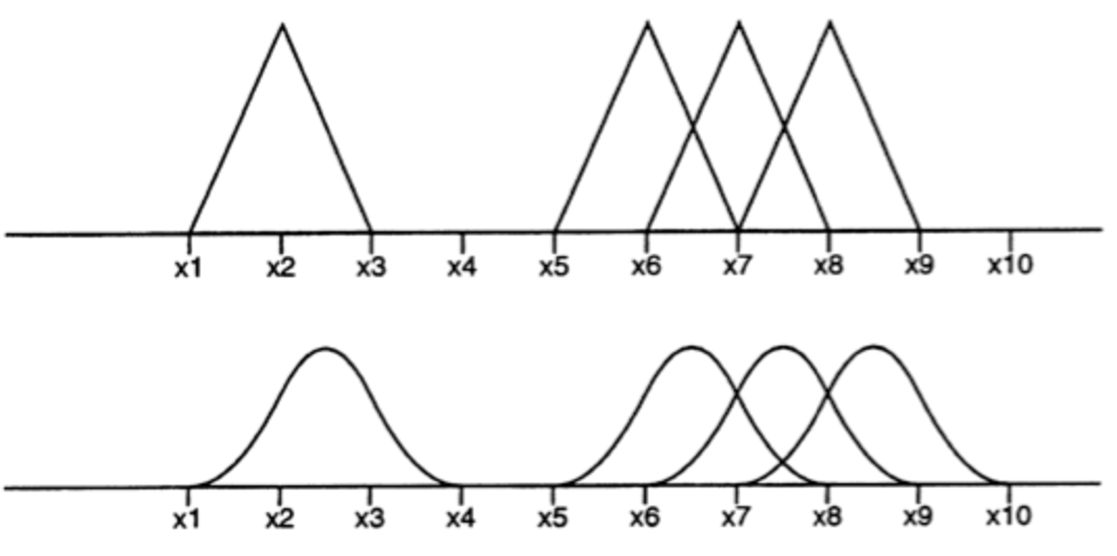
\includegraphics[width=2in]{figs/bsplines} 
%         \ec
%         \item Thin plate regression splines (Wood, 2003)
%         \bc
%         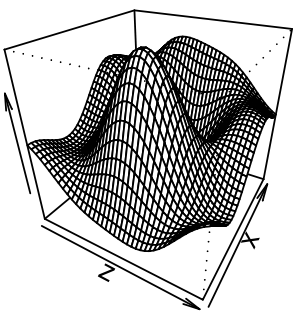
\includegraphics[width=1.25in]{figs/tprs} 
%         \ec
%        \ei
%\end{frame}




\subsection{Solutions}

\begin{frame}
	\frametitle{Proposed solutions to leakage problems}
	Two categories: PDE boundary condition based, within-area distance based.
       \bi
         \item PDEs:
	  \bi
             \item FELSPLINE (Ramsay, 2002).
             \item Soap film smoothers (Wood \emph{et al}, 2008).
           \ei
           \item Within-area distance
           \bi
             \item Geodesic Low-Rank  Thin Plate Splines (GLTPS) (Wang and Ranalli, 2007).
           \ei
        \ei
        \bc\begin{tabular}{@{}cc}
          & \\
        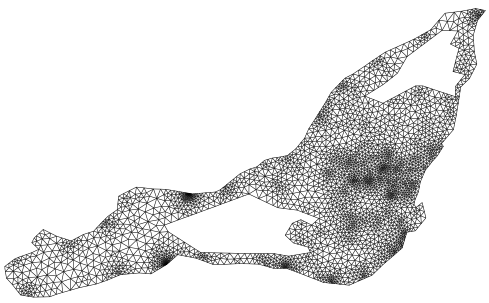
\includegraphics[width=2in]{figs/ramsaytriangulation.png}&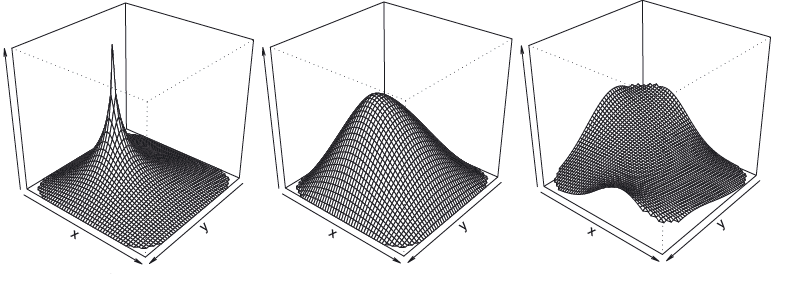
\includegraphics[width=2in]{figs/soapbases.png}\\
        \end{tabular}
        \ec
\end{frame}


\begin{frame}
	\frametitle{``The Third Way''}
      \bi
         \item Domain morphing - think of domain as silly putty.
         \item Takes into account within-area distance.
         \item Potentially less computationally intensive. 
         \item Eilers (2006) proposes Schwarz-Christoffel transform.
         \item Gives a known domain - easier to smooth over.
      \ei
      \bc
         \textbf{However:}
      \ec
      \bi
         \item Crowding - numerical singularities.
         \item Not clear what this does to the smoothness penalty - artefacts, penalty issues - but NOT GOOD!
      \ei
      \bc
         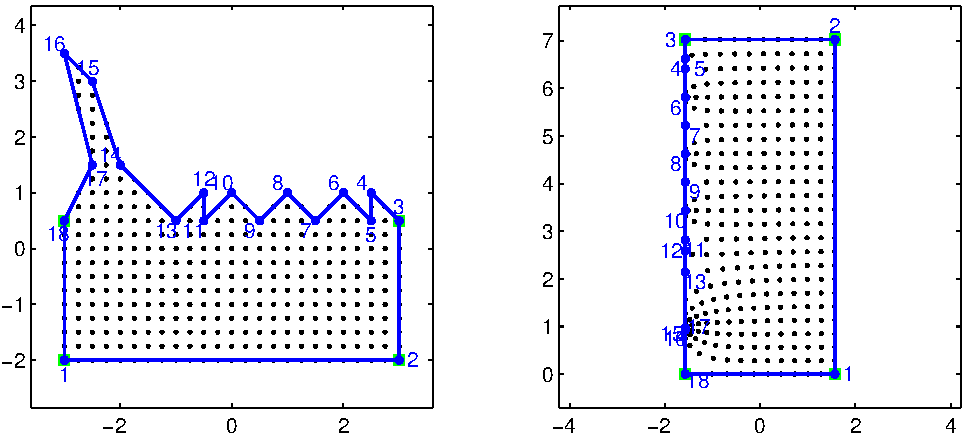
\includegraphics[height=1in]{figs/matlab-test-3}
      \ec
\end{frame}



\section{Multidimensional Scaling}

\subsection{Details}

\begin{frame}
	\frametitle{Multidimensional scaling and within-area distances}
       \bi
         \item Idea: use MDS to arrange points in the domain according to their distance within the domain.
         \ei
         \bc \textbf{Scheme:} \ec
         \bi
         \item First need to find the within-area distances.
         \item Perform MDS on the matrix of within-area distances.
         \item Find the new configuration of the points.
         \item Smooth over the new points.

        \ei
\end{frame}

\begin{frame}
	\frametitle{Multidimensional scaling refresher}
       \bi
         \item Use double centred matrix of between point distances, $D$, using the eigen-decomposition of $DD^T$ we can find new points.
         \item Finds a configuration of points such that Euclidean distance between points in new arrangement is approximately the same as distance in the domain.
          \item New points can be added into the MDS configuration via Gower's interpolation (Gower, 1968)
        \ei
            \centering
            % this is just generated from wt2-test.R
              \includegraphics[width=3in]{figs/wt2-coloured.pdf}\\
        
\end{frame}

\subsection{Finding the within-area distances}

\begin{frame}
	\frametitle{A ``new'' algorithm for finding within-area distances}

	\bc \textbf{So, how do we find the distances to put in D?}\ec
\end{frame}

\begin{frame}
	\frametitle{Finding the path - 1}
            \centering
             % trim order l b r t
              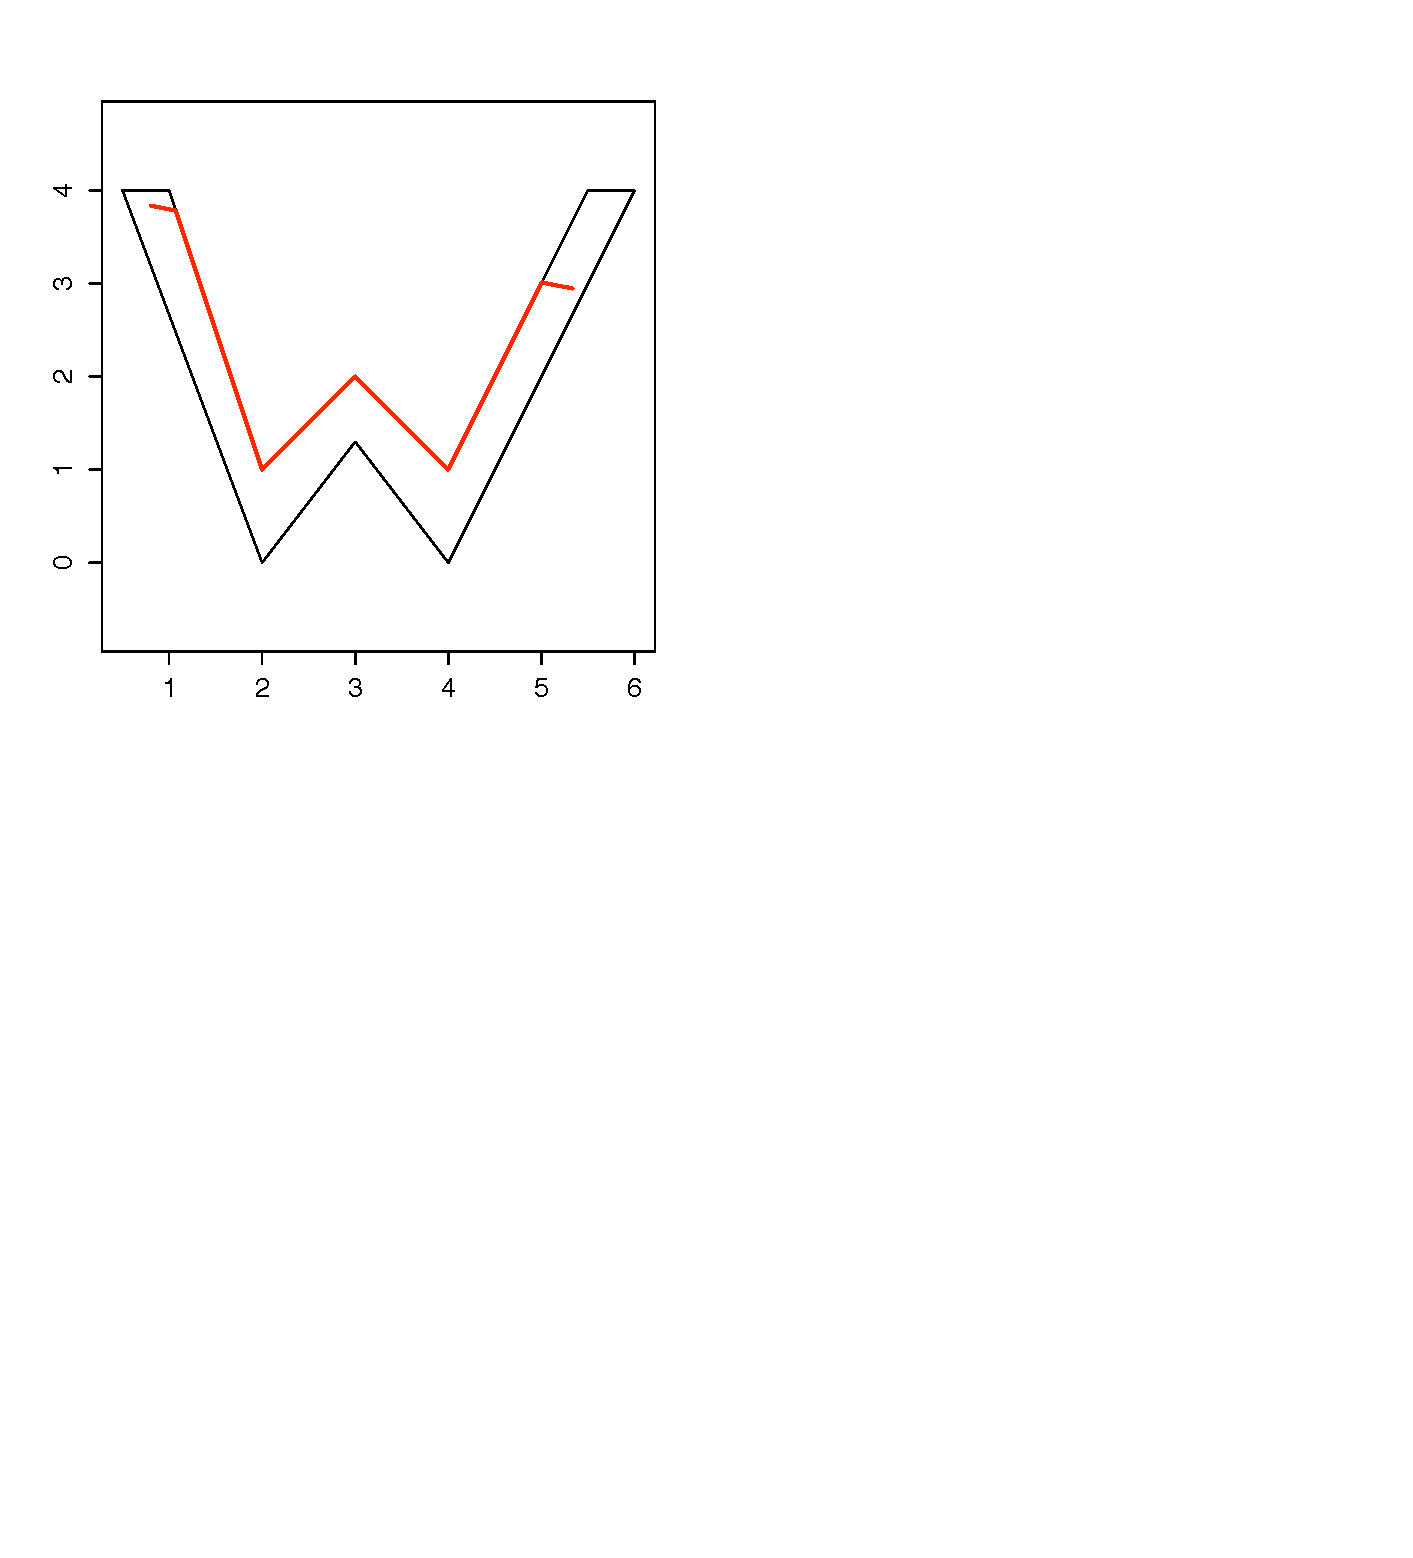
\includegraphics[width=2.75in]{figs/wood-2}\\
\end{frame}

\begin{frame}
	\frametitle{Finding the path - 2}
            \centering
              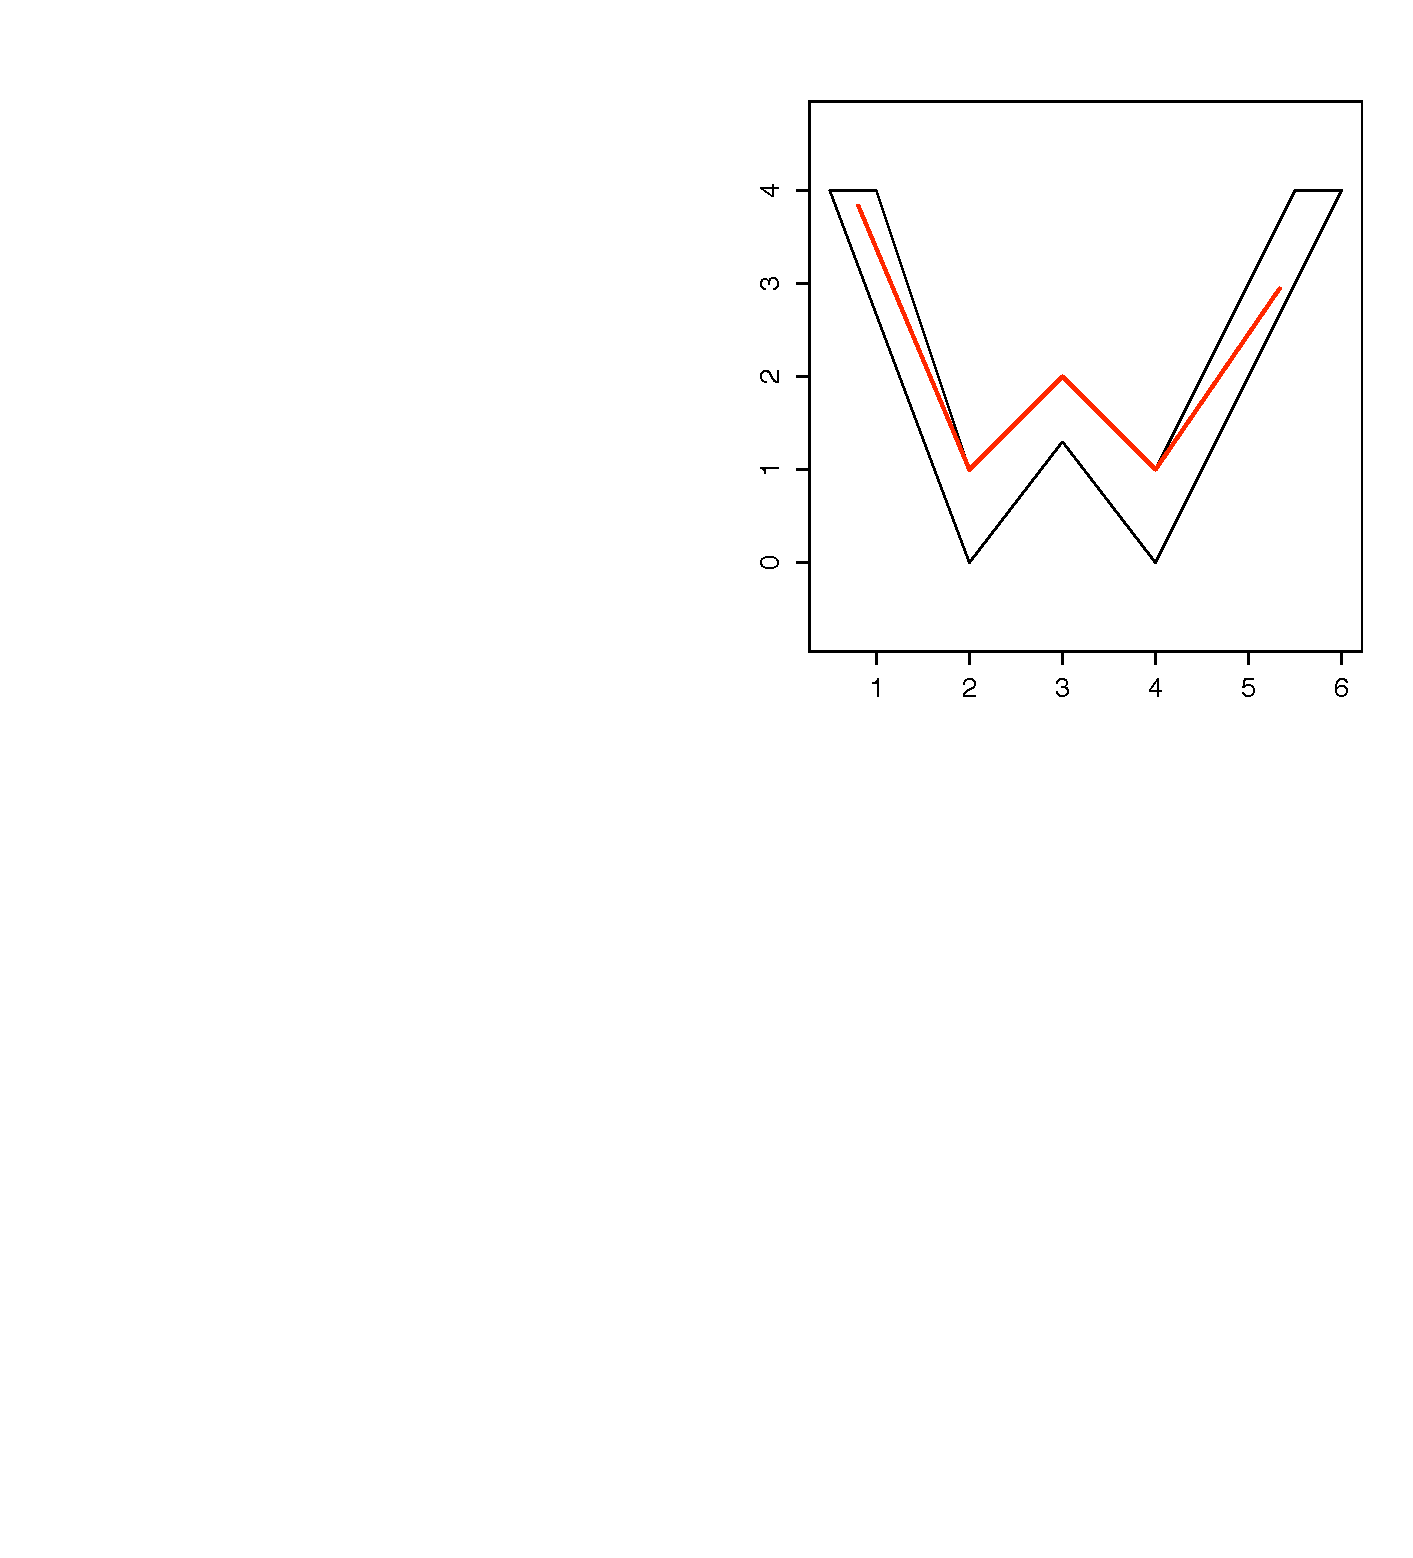
\includegraphics[width=2.75in]{figs/wood-1}\\
\end{frame}

\begin{frame}
	\frametitle{Finding the path - 3}
            \centering
              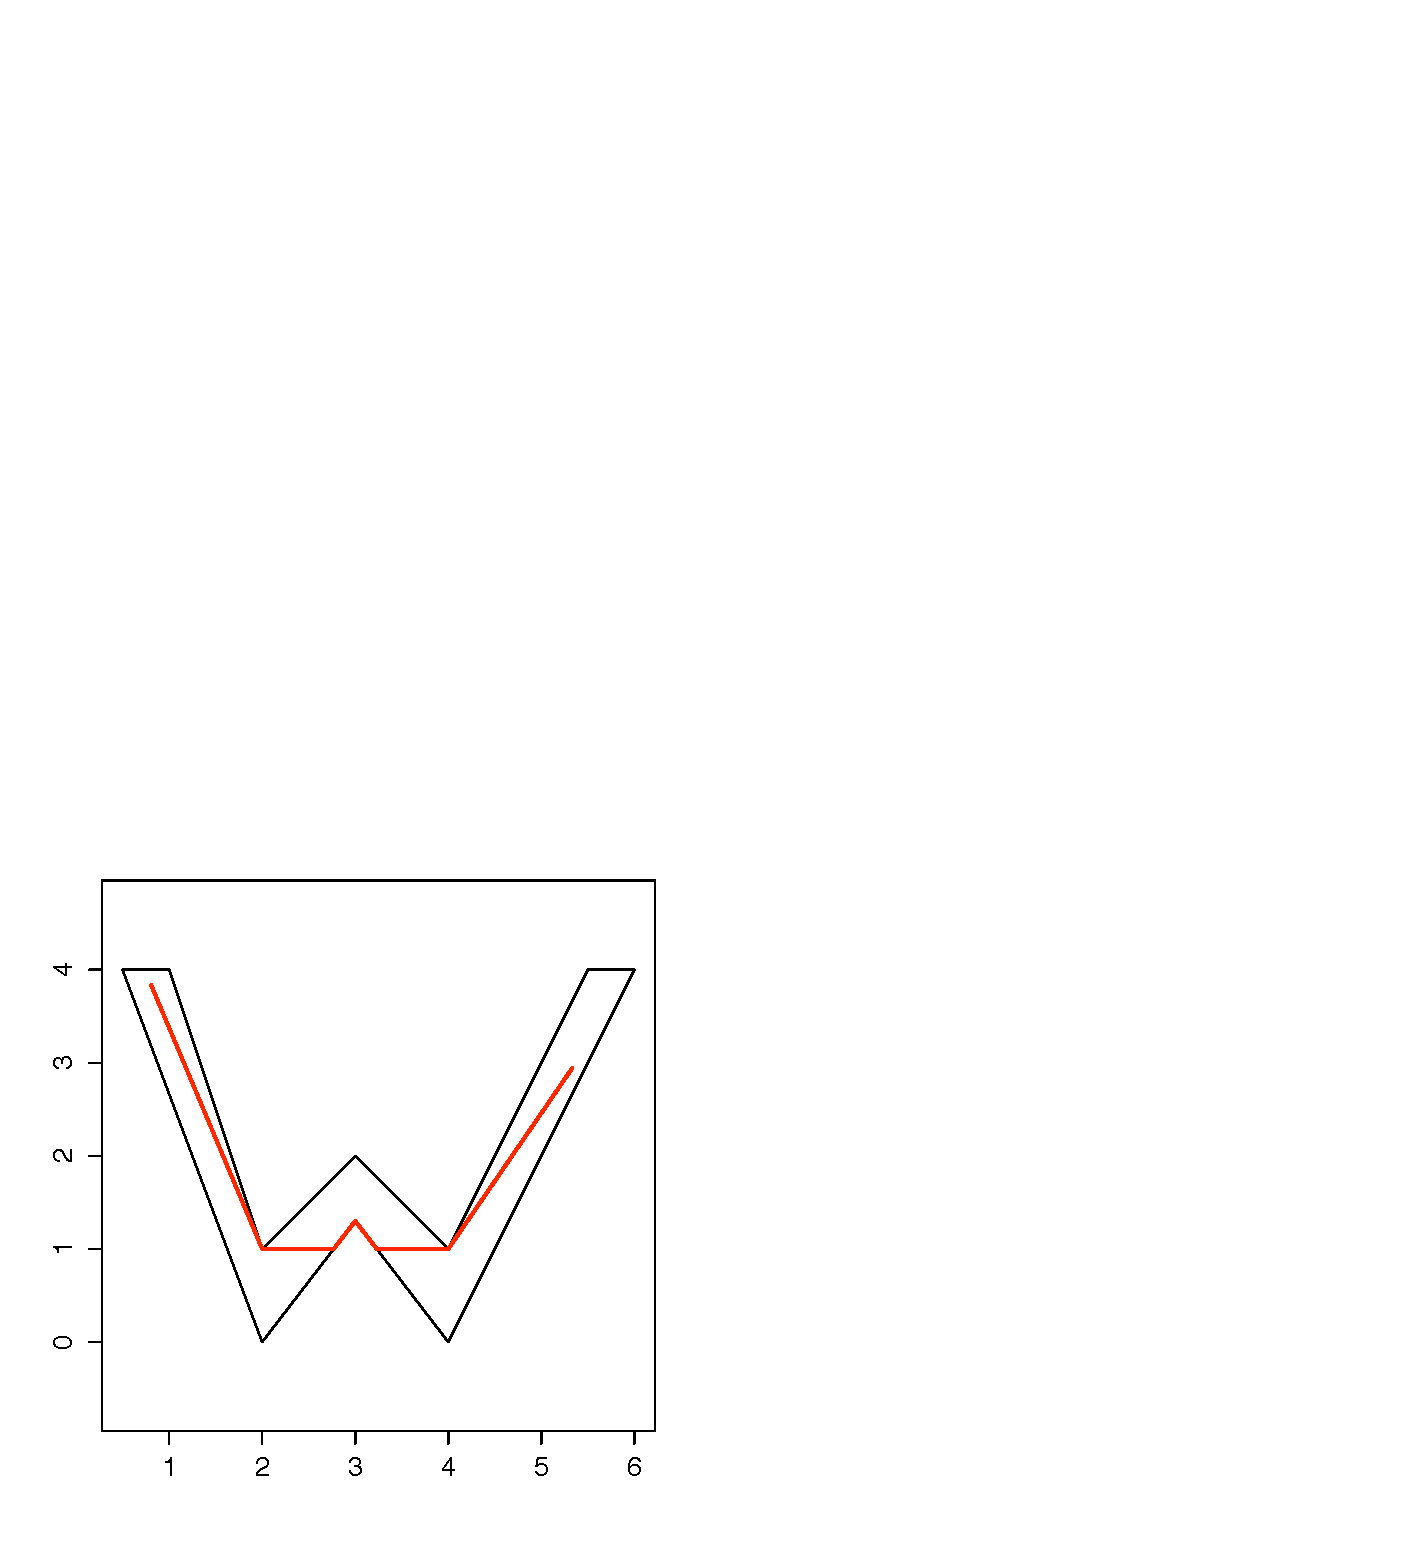
\includegraphics[width=2.75in]{figs/wood-3}\\
\end{frame}

\begin{frame}
	\frametitle{Finding the path - 4}
            \centering
              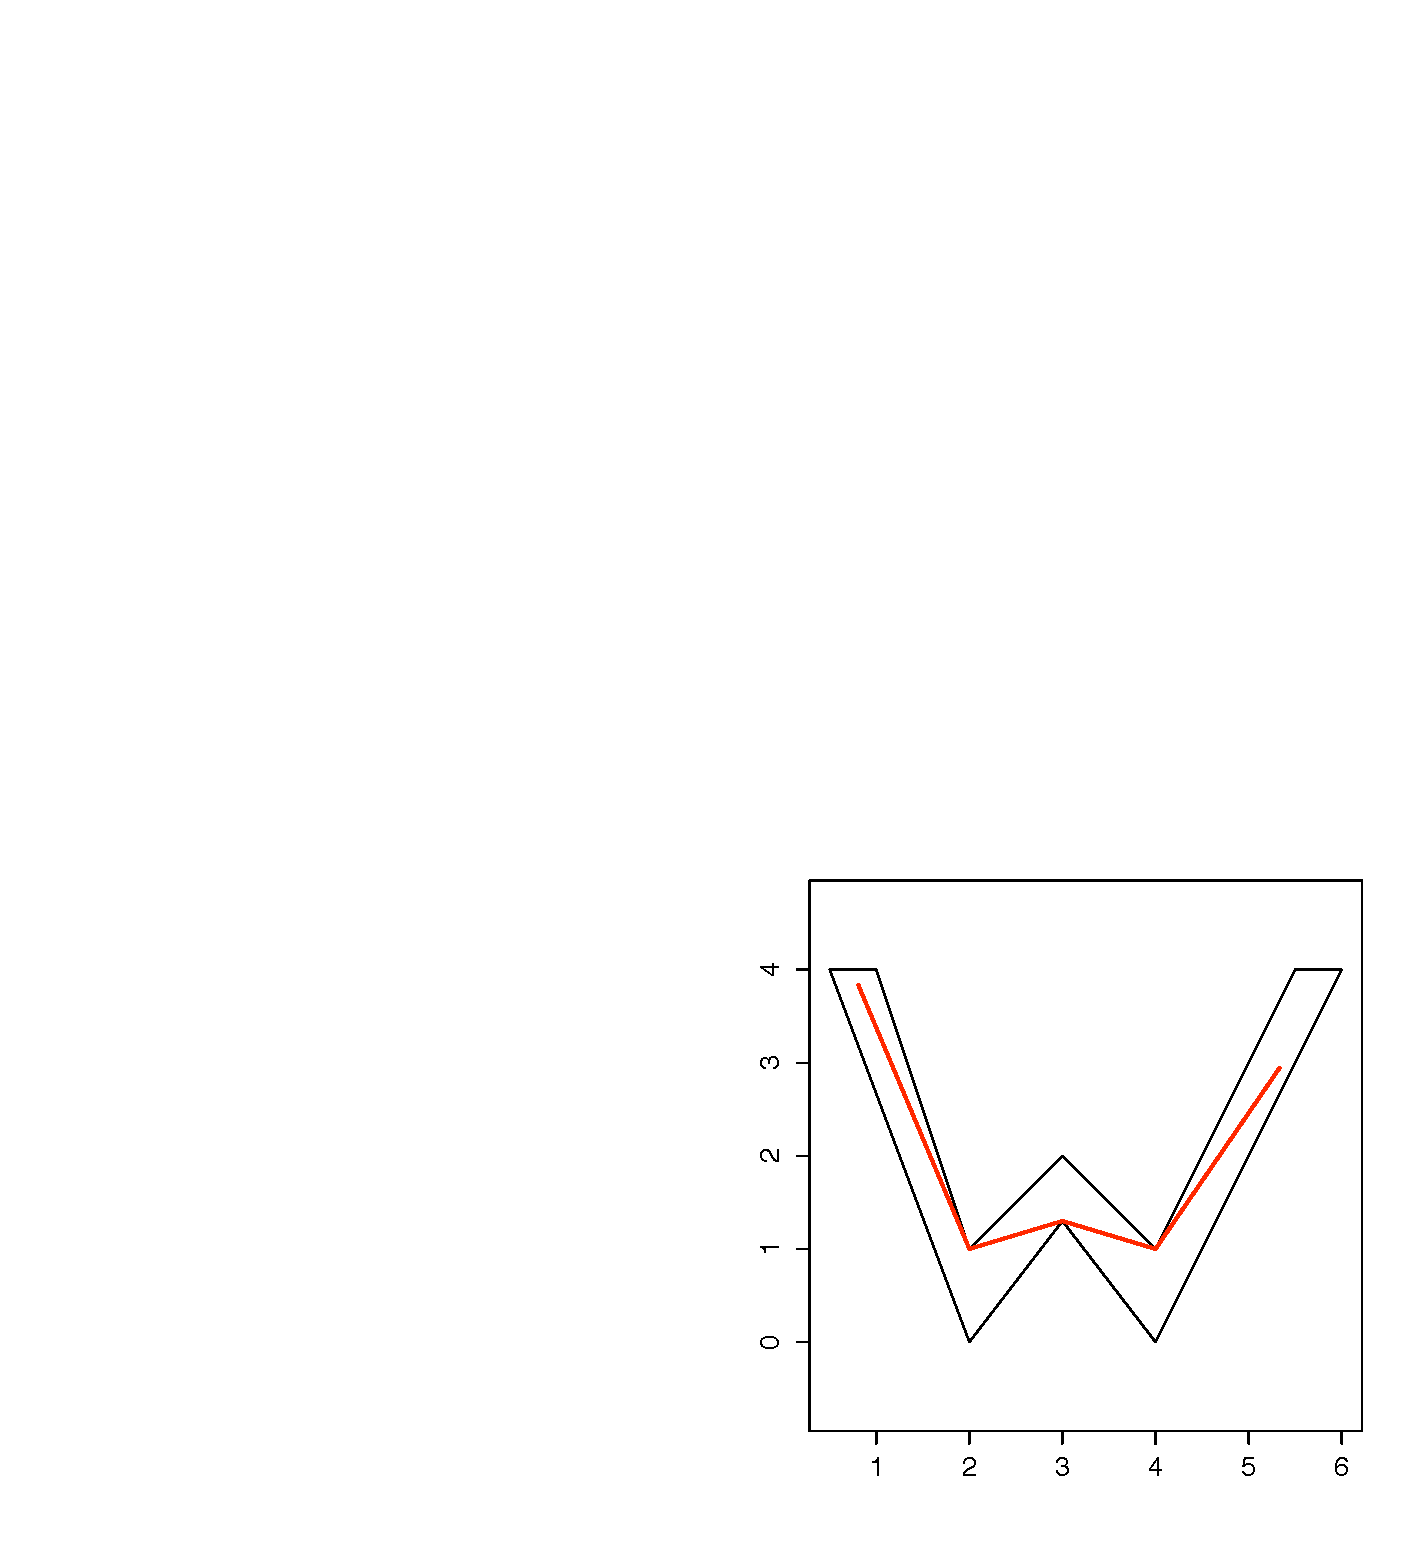
\includegraphics[width=2.75in]{figs/wood-4}\\
\end{frame}

\subsection{Simulation Results}

\begin{frame}
	\frametitle{Simulations}
	\bc \textbf{But how does it perform?}\ec
\end{frame}


\begin{frame}
	\frametitle{Ramsay simulations}
            \centering
              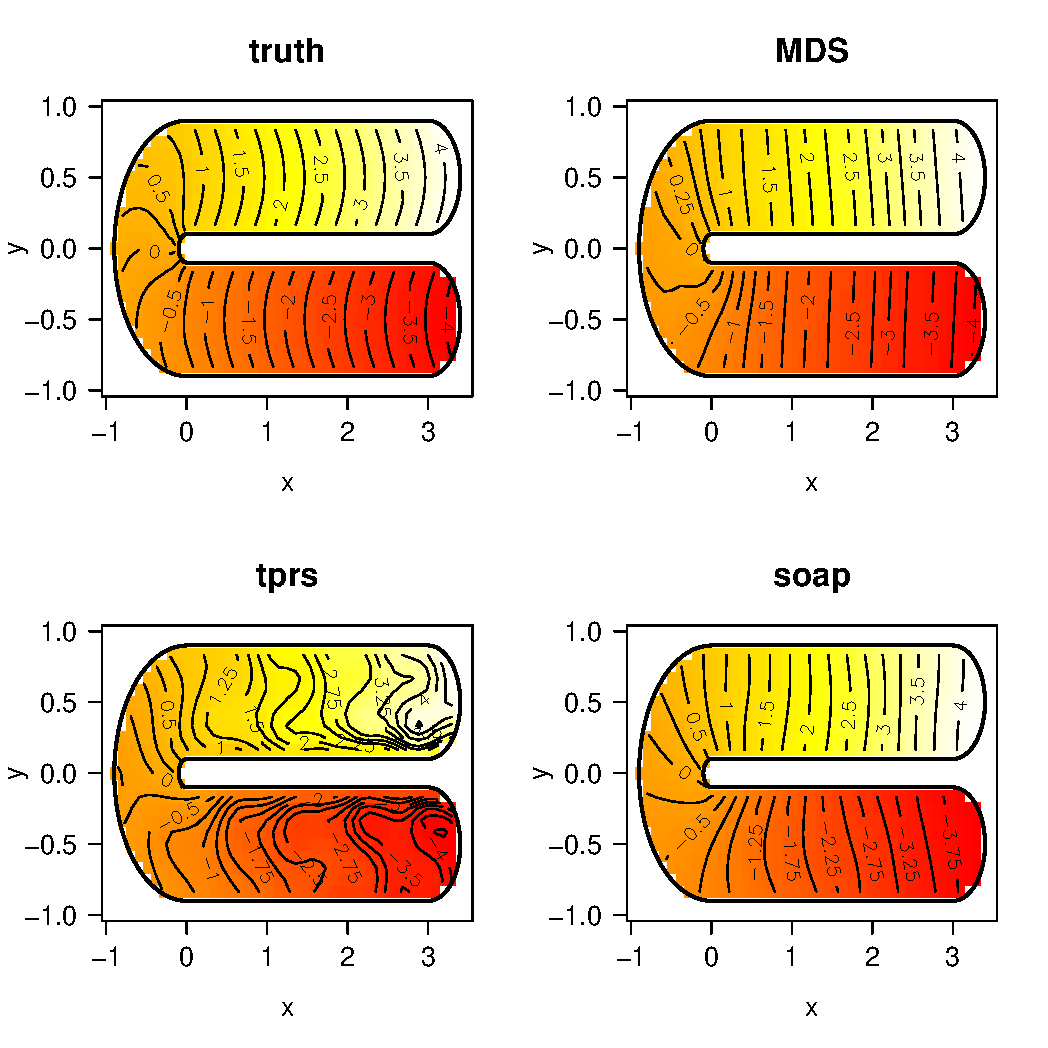
\includegraphics[width=4in]{figs/ramsay-low.pdf}\\
\end{frame}

%\begin{frame}
%	\frametitle{Ramsay simulations (high noise)}
%            \centering
%              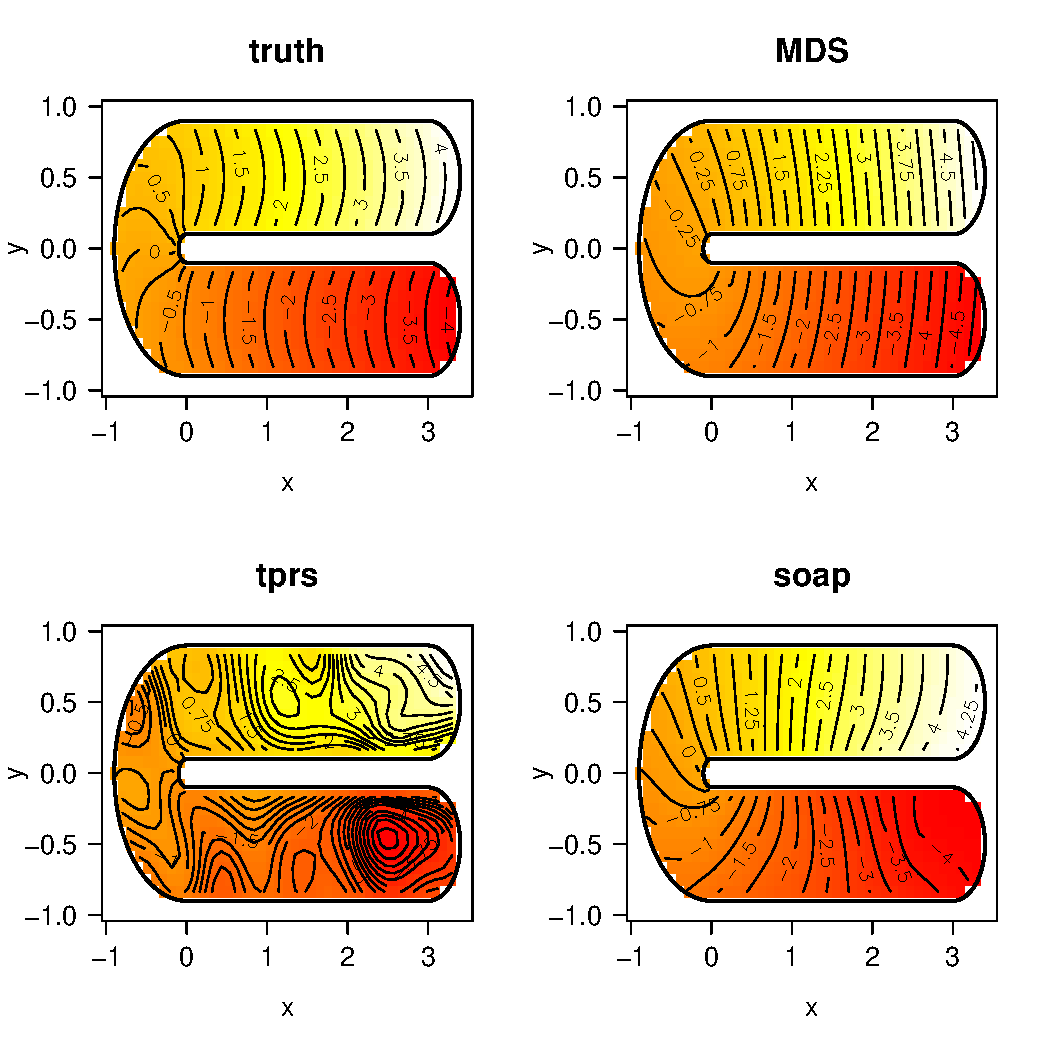
\includegraphics[width=4in]{figs/ramsay-high.pdf}\\
%\end{frame}

%\begin{frame}
%	\frametitle{A different domain}
%            \centering
%              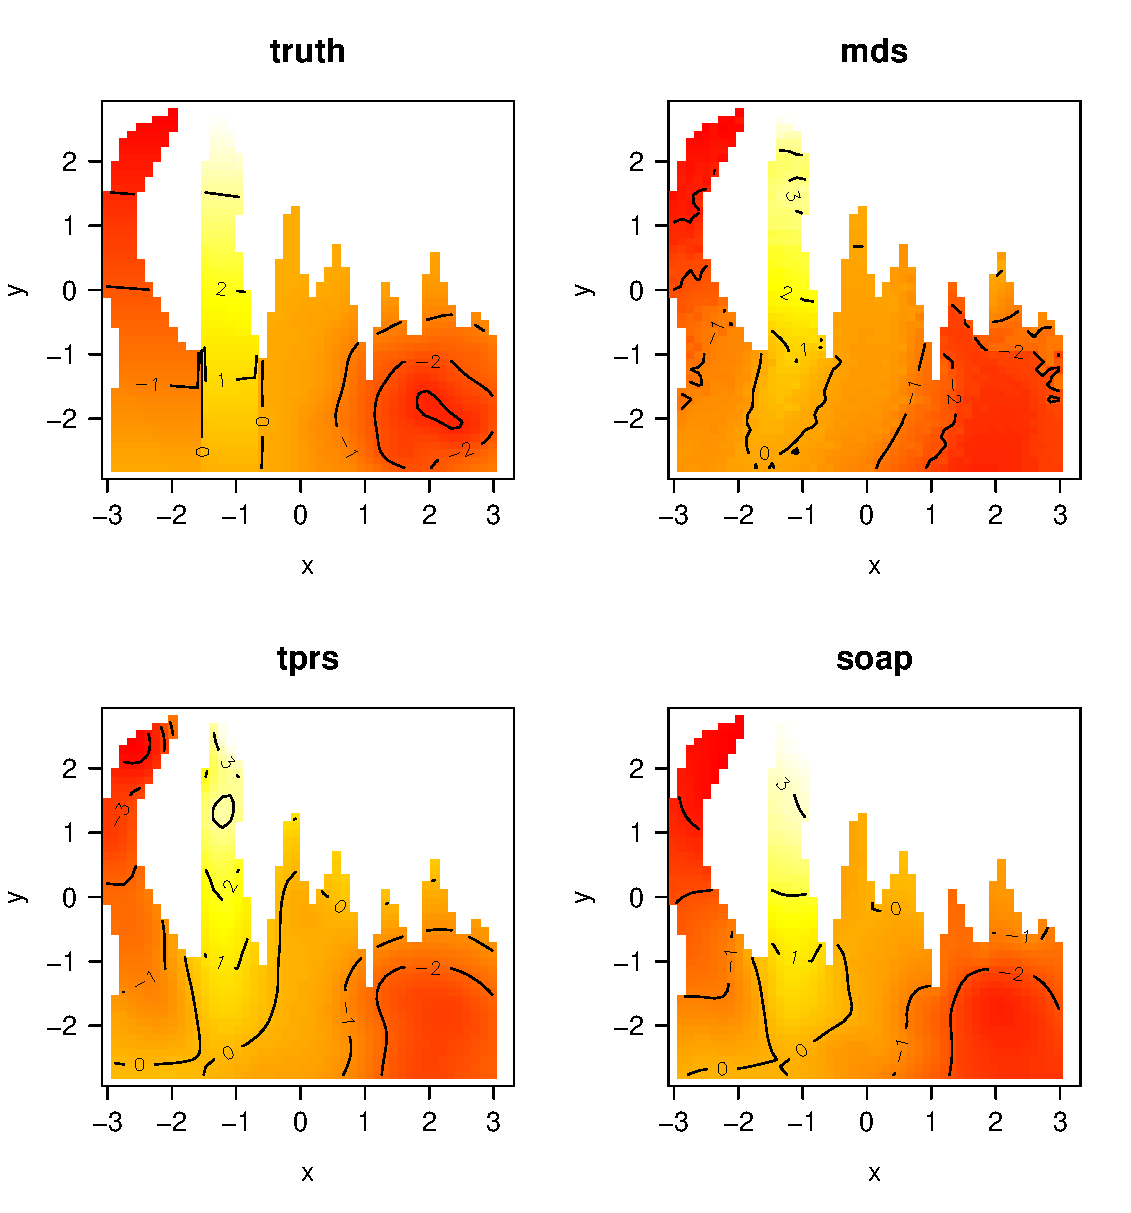
\includegraphics[width=4.5in]{figs/wt2-real.pdf}\\
%\end{frame}

\begin{frame}
	\frametitle{The Aral sea}
            \centering
              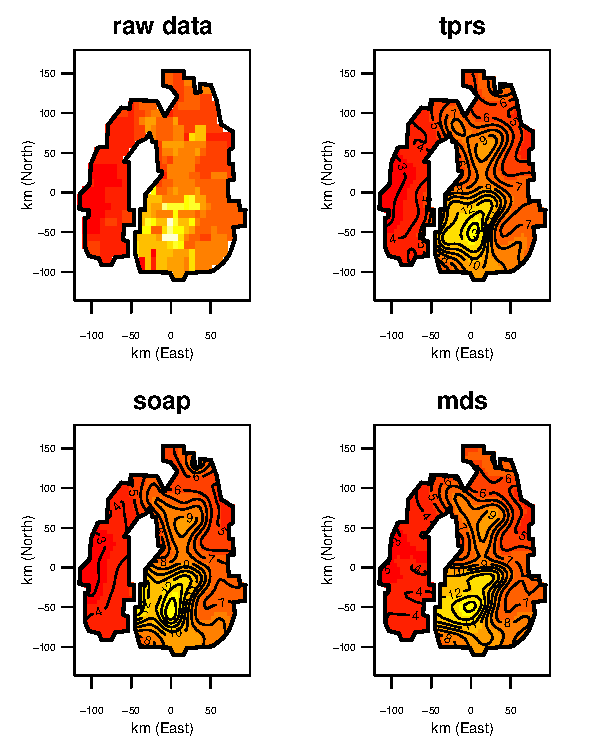
\includegraphics[height=3in]{figs/aral-fit.pdf}\\
\end{frame}

\begin{frame}
	\frametitle{So, it looks good, but...}
          \bi
            \item Computationally costly to find the within-area distances. (Esp. prediction.)
            \item Comparative in MSE terms to the soap film smoother.
            \item Artefacts.
            \item Taking a $m$-D projection of $n$-D space.
           \ei
            \centering
              \includegraphics[height=1.5in]{figs/wt2-3d-proj.pdf}\\           
\end{frame}

\begin{frame}
	\frametitle{Can we get around the squashing?}
		\bi
			\item For anisotropic smoothing, Wood (2000) suggests: 
		\ei
		\begin{equation*}
            \int\int_\Omega \Big(\frac{\partial^2 f(x,y)}{\partial x^2}\Big)^2 + k\Big(\frac{\partial^2 f(x,y)}{\partial x \partial y}\Big)^2 + k^3 \Big(\frac{\partial^2 f(x,y)}{\partial y^2}\Big)^2 \text{d}x\text{d}y.
            \end{equation*}
		\bi
			\item $\mathcal{L}^*(x,y)$, a function of point density in the new space.
              \item Adjust penalty:
          \ei
            \begin{equation*}
	            \int\int_\Omega \mathcal{L}^*(x,y) \Big( \Big(\frac{\partial^2 f(x,y)}{\partial x^2}\Big)^2 + \Big(\frac{\partial^2 f(x,y)}{\partial x \partial y}\Big)^2 + \Big(\frac{\partial^2 f(x,y)}{\partial y^2}\Big)^2\Big) \text{d}x\text{d}y.
            \end{equation*}
           \bi
           	\item Some improvements in MSE terms, doesn't get rid of all artefacts.
		\ei
\end{frame}

\begin{frame}
	\frametitle{Calculating $\mathcal{L}^*(x,y)$}
	\centering
              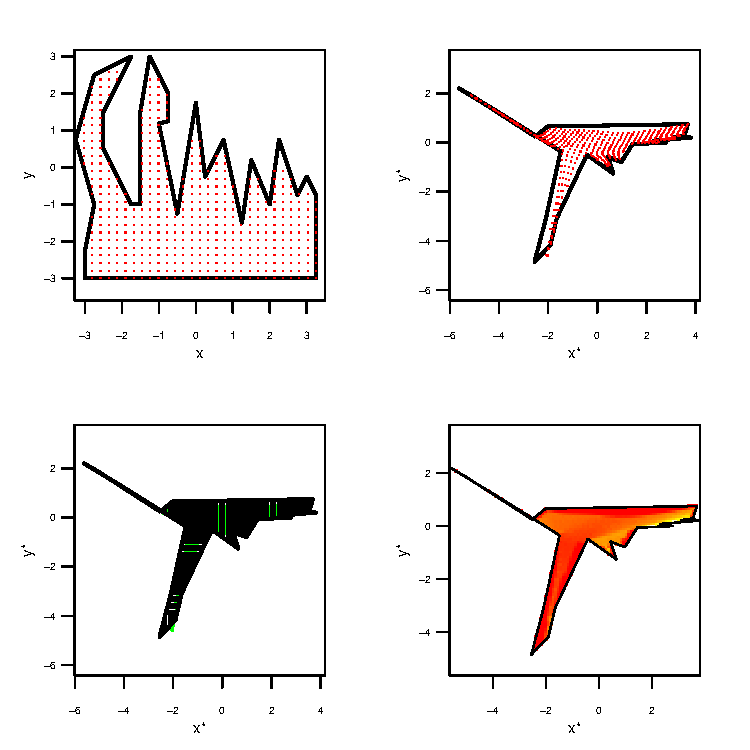
\includegraphics[height=3.5in]{figs/densgrid.pdf}
\end{frame}

\begin{frame}
	\frametitle{Ordering}
	\bi
		\item So, where are the artefacts coming from?
		\item Taking projections of $n$-dimensional space.
		\item Points can lose ordering.
		\item 3-D projection does better, but can we keep going? (Nullspace gets BIG!)
	\ei
	\centering
              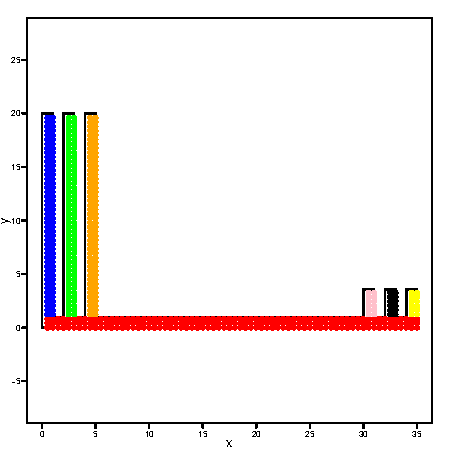
\includegraphics[height=1.75in]{figs/comb.pdf} 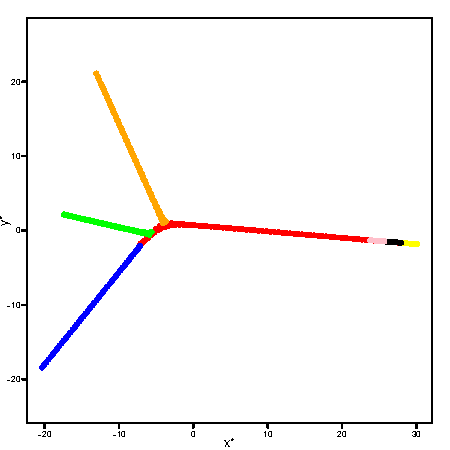
\includegraphics[height=1.75in]{figs/comb-2d.pdf}
\end{frame}

\section{Conclusions}

\begin{frame}
	\frametitle{Final comments}
		\bi
			\item Clearly, not that useful in practise.
			\item Better idea of what is required to make domain transformation work in general.
		\ei
		\textbf{Criteria for domain transformation techniques:}
          \bi
            \item Minimize squashing. No crowding.
            \item Smooth mapping.
            \item Maintain order.
            \item Fast mapping.
           \ei
         \bc \textbf{The key: transform ``just enough'' but no more.} \ec
         \bi
         		\item Smoothing on manifolds?
        \ei
\end{frame}

\begin{frame}
	\frametitle{References}
       \bi
         \item S.N. Wood, M.V. Bravington, and S.L. Hedley. \emph{Soap film smoothing. JRSSB, 2008}
         \item H. Wang and M.G. Ranalli. \emph{Low-rank smoothing splines on complicated domains. Biometrics, 2007}
         \item T.A. Driscoll and L.N. Trefethen. \emph{Schwarz-Christoffel Mapping. Cambridge, 2002}
         \item T. Ramsay. \emph{Spline smoothing over difficult regions. JRSSB, 2002}
         \item P.H.C. Eilers. \emph{P-spline smoothing on difficult domains. University of Munich seminar, 2006}
%	\item C. Chatfield and A.J. Colins. \emph{Introduction to multivariate analysis. CRC, 1980}
	\item J.C. Gower. \emph{Adding a point to vector diagrams in multivariate analysis. Biometrika, 1968.}
        \ei
        Slides available at \url{http://people.bath.ac.uk/dlm27}
\end{frame}

\begin{frame}
	\frametitle{Appendix - Ordering problems in 4-D}
	\centering
            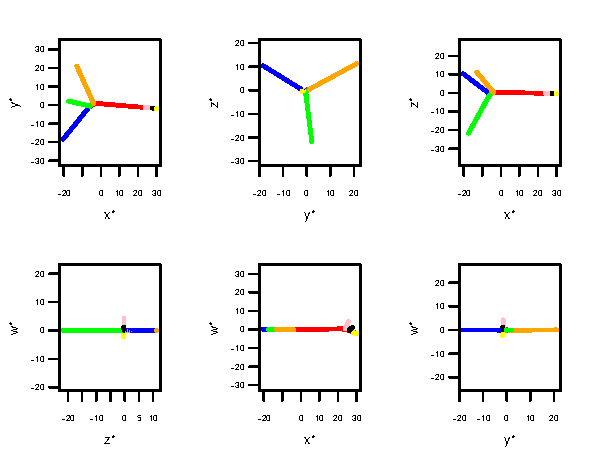
\includegraphics[height=3in]{figs/comb-4d.pdf}	
\end{frame}

\begin{frame}
	\frametitle{Appendix - A ``new'' algorithm for finding within-area distances}
	\bi
		\item Algorithm ``bounces'' around inside the polygon.
		\item Initial path is just the path around the edge, then iterate over two steps: \textit{delete} and \textit{alter}.
		\item Delete (iterating over all nodes):
			\bi \item If we can shorten the path by simply deleting a node, do that.
			\ei
		\item Alter (iterating over all nodes):
			\bi \item If we can find a shorter sub-path by bouncing off the other ``side'' of the polygon, do that.
			\ei
	\ei
\end{frame}


\end{document}
